% Makros zur Kompatibilitaet mit Onlinemodul: 
 \providecommand{\MoIl}[1][]{\mbox{}#1]\mathopen{}} 
 \providecommand{\MoIr}[1][]{#1[\mbox{}} 
 \providecommand{\MIntvlSep}{;} 
 \providecommand{\MElSetSep}{\, ; \, } 
 \begin{MAufgabe}{Lineare Betrags(un)gleichungen}{vr, 2016, MaTeX}
L\"osen Sie die Gleichung
$$
 \MDS 2\left| 6\, x + 3 \right|+4\, x - 4= 5 \left|  - 3\, x - 3 \right| -1
$$  

\ifLsg\MLoesung

Im ersten Schritt k\"onnen die Terme au\ss{}erhalb der Betragszeichen zusammengefasst werden:

\begin{align*} 
 2\left| 6\, x + 3 \right|+4\, x - 4= 5 \left|  - 3\, x - 3 \right| -1\\ 
\Leftrightarrow4\, x - 5\, \left|3\, x + 3\right| + 2\, \left|6\, x + 3\right| - 3= 0 
 \end{align*}

F\"ur diese Gleichung haben wir 4 F\"alle zu unterscheiden: 
\begin{enumerate}
\item $ \MDS 
\begin{cases} 
 0 \leq 6\, x + 3\\ 
0 \leq  - 3\, x - 3
 \end{cases}
 \mbox{ : keine L\"osung. Diese Bedingung ist nirgendwo erf\"ullt.}$ 
\item $ \MDS 
\begin{cases} 
 0 \leq 6\, x + 3\\ 
 - 3\, x - 3 < 0
 \end{cases}
\Leftrightarrow - \frac{1}{2} \leq x\Leftrightarrow x \in [ - \frac{1}{2} \, \MIntvlSep \, \infty\MoIr $ 
\item $ \MDS 
\begin{cases} 
 6\, x + 3 < 0\\ 
0 \leq  - 3\, x - 3
 \end{cases}
\Leftrightarrow x \leq -1\Leftrightarrow x \in \MoIl  -\infty \, \MIntvlSep \, -1]$ 
\item $ \MDS 
\begin{cases} 
 6\, x + 3 < 0\\ 
 - 3\, x - 3 < 0
 \end{cases}
\Leftrightarrow -1 < x \wedge x < - \frac{1}{2}\Leftrightarrow x \in \MoIl  -1 \, \MIntvlSep \, - \frac{1}{2}\MoIr $ 
\end{enumerate} 
Der 1. Fall ist nirgendwo erf\"ullt. Betrachte weiter nur die restlichen F\"alle.
 
 Fallunterscheidung: 

 \begin{enumerate} 
 \item Sei $ \MDS x\in[ - \frac{1}{2} \, \MIntvlSep \, \infty\MoIr $. 
 In diesem Fall gilt: 
  $ \MDS \left| 6\, x + 3\right|=6\, x + 3$ und $ \MDS \left|  - 3\, x - 3\right|=3\, x + 3$. \\ 
 Damit ist die Gleichung 
 $$ 
4\, x - 5\, \left|3\, x + 3\right| + 2\, \left|6\, x + 3\right| - 3= 0
$$
 \"aquivalent zur Gleichung
 $$ 
2\left(6\, x + 3\right)-5\left( 3\, x + 3\right)+4\, x-3= 0 
$$  
$$ 
 \Leftrightarrow x - 12= 0 
$$  
$$ \Leftrightarrow x = 12 . 
 $$ 
 Die L\"osung muss auch die Fallbedingung $x\in [ - \frac{1}{2} \, \MIntvlSep \, \infty\MoIr  $ erf\"ullen. Die gefundene L\"osung $x=12$ erf\"ullt die Fallbedingung  $x\in [ - \frac{1}{2} \, \MIntvlSep \, \infty\MoIr $ und deshalb ist  $$
 \mathcal{L}_{1}=\left\{12\right\}
 $$ 
\item Sei $ \MDS x\in\MoIl  -\infty \, \MIntvlSep \, -1]$. 
 In diesem Fall gilt: 
  $ \MDS \left| 6\, x + 3\right|= - 6\, x - 3$ und $ \MDS \left|  - 3\, x - 3\right|= - 3\, x - 3$. \\ 
 Damit ist die Gleichung 
 $$ 
4\, x - 5\, \left|3\, x + 3\right| + 2\, \left|6\, x + 3\right| - 3= 0
$$
 \"aquivalent zur Gleichung
 $$ 
2\left( - 6\, x - 3\right)-5\left(  - 3\, x - 3\right)+4\, x-3= 0 
$$  
$$ 
 \Leftrightarrow 7\, x + 6= 0 
$$  
$$ \Leftrightarrow x = - \frac{6}{7} . 
 $$ 
 Die L\"osung muss auch die Fallbedingung $x\in \MoIl  -\infty \, \MIntvlSep \, -1] $ erf\"ullen. Die gefundene L\"osung $x=- \frac{6}{7}$ erf\"ullt die Fallbedingung  $x\in \MoIl  -\infty \, \MIntvlSep \, -1]$ nicht und deshalb ist  $$
 \mathcal{L}_{2}=\emptyset 
 $$ 
\item Sei $ \MDS x\in\MoIl  -1 \, \MIntvlSep \, - \frac{1}{2}\MoIr $. 
 In diesem Fall gilt: 
  $ \MDS \left| 6\, x + 3\right|= - 6\, x - 3$ und $ \MDS \left|  - 3\, x - 3\right|=3\, x + 3$. \\ 
 Damit ist die Gleichung 
 $$ 
4\, x - 5\, \left|3\, x + 3\right| + 2\, \left|6\, x + 3\right| - 3= 0
$$
 \"aquivalent zur Gleichung
 $$ 
2\left( - 6\, x - 3\right)-5\left( 3\, x + 3\right)+4\, x-3= 0 
$$  
$$ 
 \Leftrightarrow  - 23\, x - 24= 0 
$$  
$$ \Leftrightarrow x = - \frac{24}{23} . 
 $$ 
 Die L\"osung muss auch die Fallbedingung $x\in \MoIl  -1 \, \MIntvlSep \, - \frac{1}{2}\MoIr  $ erf\"ullen. Die gefundene L\"osung $x=- \frac{24}{23}$ erf\"ullt die Fallbedingung  $x\in \MoIl  -1 \, \MIntvlSep \, - \frac{1}{2}\MoIr $ nicht und deshalb ist  $$
 \mathcal{L}_{3}=\emptyset 
 $$ 
 \end{enumerate} 
  Die L\"osungsmenge des Ausgangsproblems ist die Vereinigung der einzelnen L\"osungsmengen: 
$$ \mathcal{L} = \mathcal{L}_{1} \cup \mathcal{L}_{2} \cup \mathcal{L}_{3} 
 = \left\{12\right\}\cup \emptyset\cup \emptyset 
  =\left\{12\right\} 
   . $$ 
 
 \begin{center}
 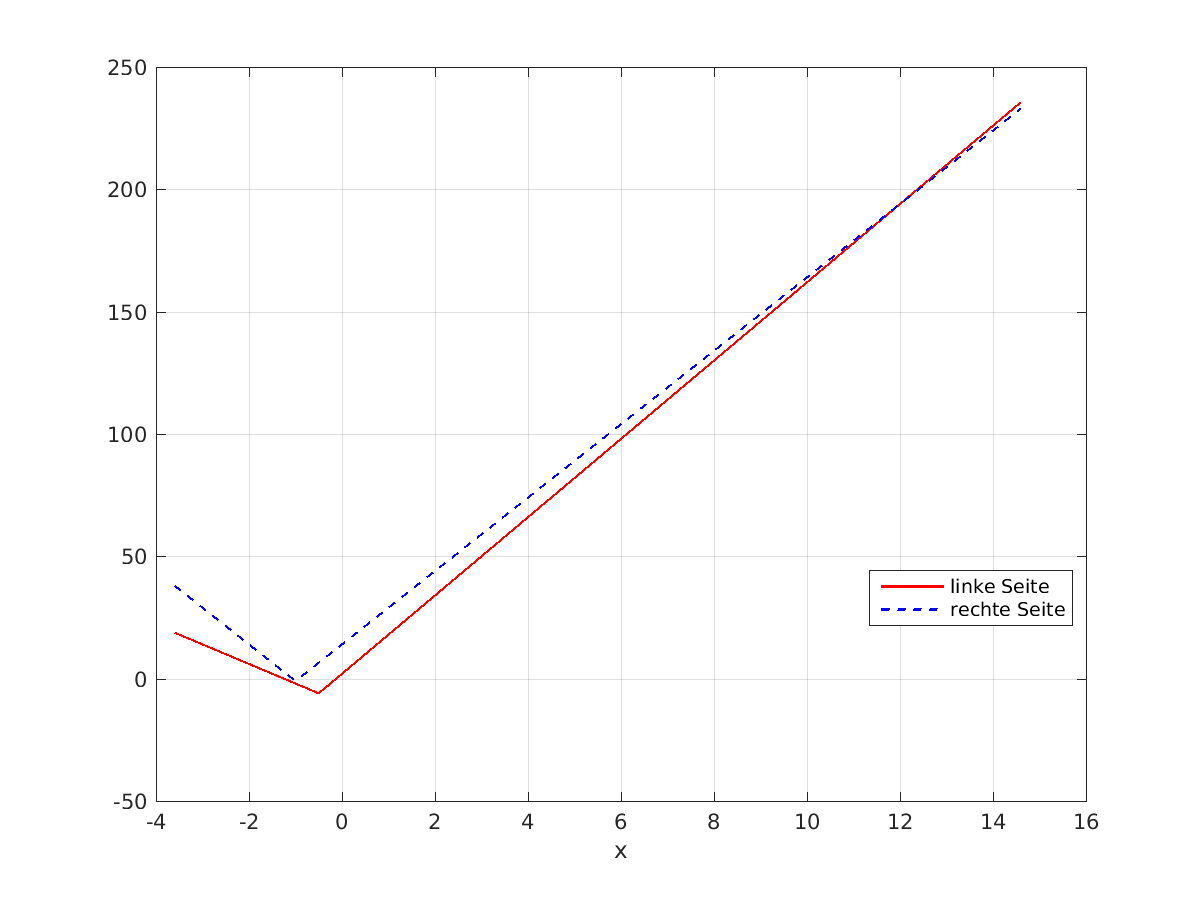
\includegraphics[width=0.8\linewidth]{Abb_zur_Ag_autogenerated_ineq_1.png} \end{center}
 
\else\relax\fi
 \end{MAufgabe}